\chapter{NMF in speech processing}  %Title of the First Chapter



Non-Negative matrix decomposition or factorization is an algorithm where the objective is to approximate the given non-negative data matrix  $V \in \mathbb{R}^{\geq 0, M \times N}$ as a product of two non-negative matrices. the basis vector matrix,  $W \in \mathbb{R}^{\geq 0, M \times R}$ and the activation matrix $H \in \mathbb{R}^{\geq 0, N \times R}$.The parameter $R$ specifies the rank of the decomposition and depends on the complexity of the matrix $V$ that is being decomposed. NMF has been widely used in audio processing where it is applied on the magnitude spectrogram. The Magnitude spectrogram is inherently non-negative, and thus lends itself well to the NMF algorithm.
Since the problem of NMF does not have an analytical solution, a numerical approximation is generally used. Specifically, an objective function is chosen that quantifies the approximation error and using the gradient descent algorithm, minimum error is achieved. Thus, the NMF problem can be modeled as a constrained optimization problem, where the objective is to minimize the error of reconstruction of the original data matrix $V$. In this chapter, the Kullback-Leiber divergence has been used to measure the error since it has a special significance for speech spectrograms. It is defined as - 

\begin{align}
D = \left \| V \odot ln \left (  \frac{V}{W.H} \right ) -V +W.H \right \| \label{kldiv}
\end{align}
 $\left \| \cdot  \right \|_F$ in the Forbenious norm, $V$ is the data matrix being factorized and $W$ and $H$ are the factors.
This error has to minimized subject to the non-negativity constraints to achieve an accurate approximation. Thus, this is a contrained optimization problem. In \cite{lee} a multiplicativs update rules for $W$ and $H$ matrices that assures convergence to minimum error. They as given as
\begin{align}
H = H \odot \frac{W^T \cdot \frac{V}{W\cdot H} }{W^T\cdot 1} \label{H updates}
\end{align}
\begin{align}
W = W \odot \frac{\frac{V}{W\cdot H}\cdot H^T   }{ 1 \cdot H^T} \label{W updates}
\end{align}

$ \odot $ is the Hamdard product, all divisions are element wise and $1$ is a $M \times N$ matrix with all elements set to 1.

The steps to calculating the Non-Negative matrix factorization of a given data matrix, $V$ are given as -
\begin{itemize}
\item Randomly initialize the $W \in \mathbb{R}^{\geq 0, M \times R}$ and $H \in \mathbb{R}^{\geq 0, N \times R}$ with non negative values and with an appropriate value for the rank of the decomposition $R$
\item Apply multiplicative updates to the matrices as in Equations \ref{H updates} and \ref{W updates}  and calculate error at every iteration.
\item Stop after the error is lesser than a present threshold. Since the error converges to a finite positive value which will be unknown before the decomposition, and a relatively small tolerance level might not let the algorithm terminate,  it is advisable to use the number of iterations as a parameter to set the endpoint for the algorithm. 
\end{itemize}


\section{Illustration of NMF for audio}
In Figure 2.1, shows the spectogram of an instrumental piece of music, played on a piano, with 4 distinct notes, some played multiple  times. The duration of the audio is 4.7 seconds and has been sampled at $16kHz$. NMF was applied on ,$V$, the magnitude spectrogram of the audio signal, shown in Figure 2.1. Figure 2.2 shows the spectrogram of $\hat{V} \approx W.H$. The number of basis vectors ($R$) was chosen to be 5 and NMF was allowed 100 iterations.

Visually, it seems apparent that NMF has done a good job of representing the spectrogram with a limited number of basis. The reconstructed audio has no perceptible artifacts \cite{A}.  This is to be expected because the data has a simple structure in terms of the temporal patterns in the spectrogram. The structure is due to the fact that non-percussion instruments like the piano have a finite number of notes and each note has a unique fundamental frequency and predefined harmonics.These qualities do not extend to speech signals. This makes it difficult for the conventional NMF approach to do well in the speech scenario.

The two matrices, $W$ and $H$ have special significace when NMF is applied to the magnitude spectrogram. $W$ is the matrix whose columns are the basis set for $\hat{V}$. $H$ is a stack of set of row $R$ row vectors that constitute the weights corresponding to each basis vector across the time axis of the magnitude spectrogram. $W$ is called the basis vector matrix and $H$ is called the activation matrix, since it determines where on the time axis of the manitude spectrogram, a particular basis vector is 'activated'.





\begin{figure}
\centering
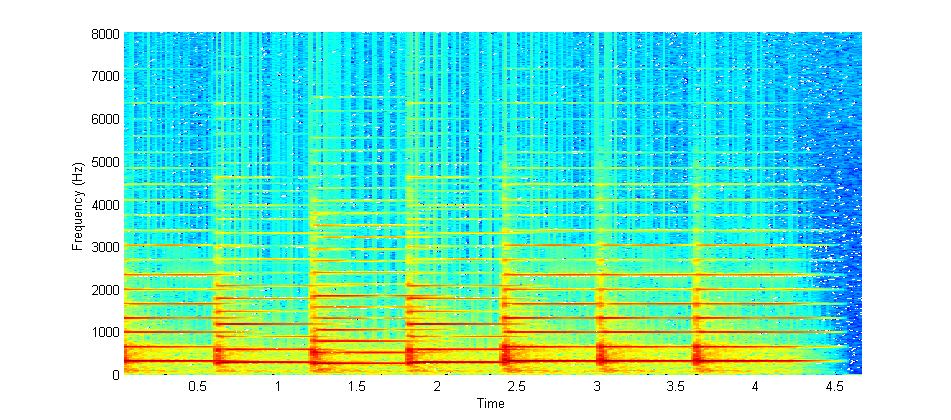
\includegraphics[scale=0.4]{mary_spectrogram}
\caption{Spectrogram of \emph{Mary}. Key STFT parameters - Sampling frequency : $16000kHz$. Window : hanning window of length 1024 samples. Overlap : 756 samples. FFT size 1024}
\end{figure}


\begin{figure}
\centering
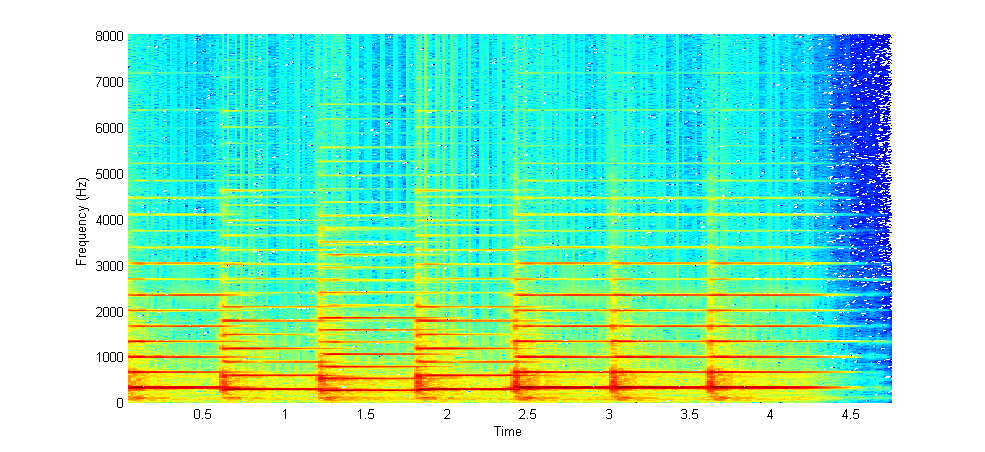
\includegraphics[scale=0.4]{mary_recon_spectrogram}
\caption{Reconstructed Spectrogram of \emph{Mary}. Key STFT parameters - \textbf{Sampling frequency} : $16000kHz$. \textbf{Window} : hanning window of length 1024 samples. \textbf{Overlap} : 756 samples. \textbf{Size of fft}: 1024 }
\end{figure}

\begin{figure}
\centering
\begin{minipage}{.5\textwidth}
  \centering
  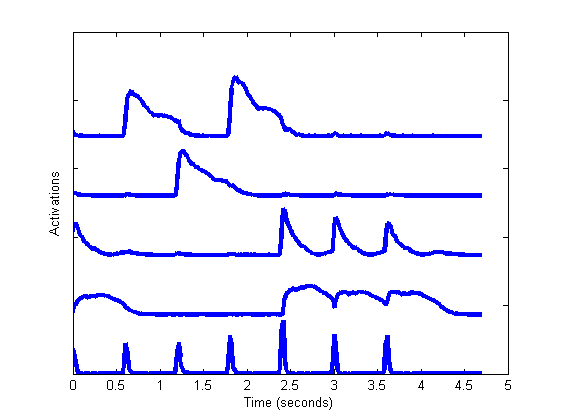
\includegraphics[width=.9\linewidth]{activations_mary}
  \captionof{figure}{The activation vectors corresponding to each basis vector}
  \label{fig:test1}
\end{minipage}%
\begin{minipage}{.5\textwidth}
  \centering
  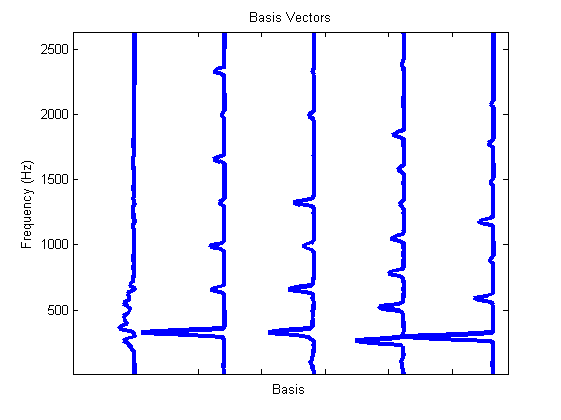
\includegraphics[width=.9\linewidth]{basis_vectors_mary}
  \captionof{figure}{Basis vectors. A total of 5 basis vectors were used. A zoomed version is shown to show the differences in frequencies}
  \label{fig:test2}
\end{minipage}
\end{figure}

Figure 2.3 and 2.4 show the activation times for each basis vector and the the basis vectors respectively. The activation vectors for the basis vectors from left to right are shown from bottom to top. It should be noted that the basis vectors are in fact magnitude spectra.\\

Refering to Figure 2.3 and 2.4, and analysing the activation times, we find that we can map them to the pattern of playing of a specific note at particular time instants. For example, the rightmost basis vector in the Figure 2.4 (corresponding to the topmost activation vector in Figure 2.3) gets activated at two time instants which are actually approximately the times of playing of a single specific note in the audio. It can also be seen that no other basis vector is getting activated during the period of activation of this basis vector. It follows that this basis vector has captured the expression of this note in the spectrogram. This is made clear when the audio reconstruction of the spectrogram achieved by setting all other activations to zero is heard \cite{A}. \\
Not all basis vectors though capture single notes this cleanly. Looking at the activations, it is also evident that the basis vectors corresponding to two activations (3rd and 4th from the top) get activated together whenever a particular note is played. To get the full expression of this note, we need both these basis vectors. \\
Also, the basis vector corresponding the the bottom most activation vector does not represent any single note, but is activated at the times of change of note. It can be inferred that this basis vector represents the complex part of the spectra when a note is just struck and the power is spread throughout the spectrum, just like in a percussion instrument.

\section{Convolutive NMF}
Figures 2.5-2.6 correspond to an audio sample, \emph{Machali}\cite{A}. It is an audio which is a speech recording of the sentence, \emph{"Machali jal ki hai rani, jeevan uska hai paani"}, in Hindi. It is 4.7 seconds long and is sampled at 16kHz. The figures  represent the magnitude spectrogram of the original audio, the reconstructed spectrogram via NMF using $R = 8$, the activation matrix and the basis vectors, in that order. Although the duration of the audio is the same as \emph{Mary}, to achieve the same accuracy, we need 8 basis vectors to represent the magnitude spectra. This is intuitive since speech signals have complex spectrogram patterns and thus have a higher rank than that of an instrumental piece, like \emph{Mary}.

\begin{figure}
\centering
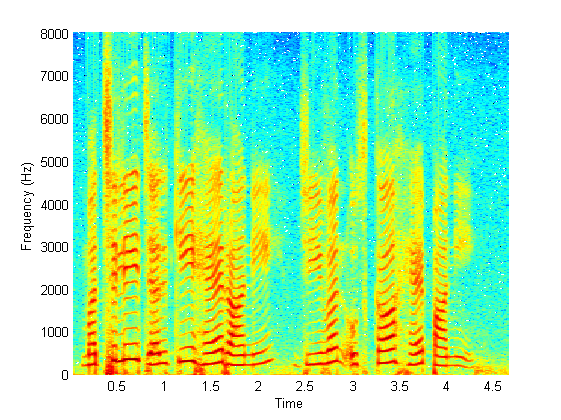
\includegraphics[scale=0.6]{machali_spectrogram}
\caption{Spectrogram of \emph{Machali}. Key STFT parameters - Sampling frequency : $16000kHz$. Window : Hanning window of length 1024 samples. Overlap : 756 samples. Size of fft: 1024 } \label{machali_spectrogram_ch2}
\end{figure}

\begin{figure}
\centering
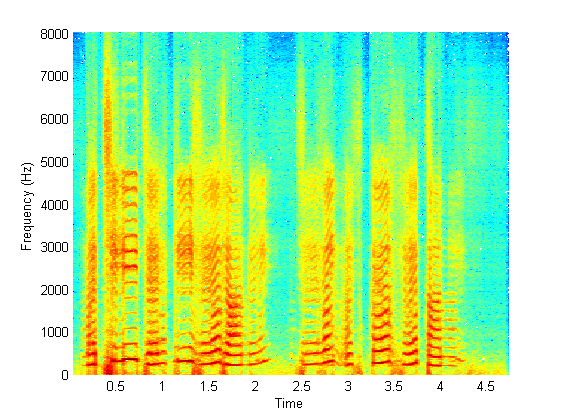
\includegraphics[scale=0.6]{machali_recon_spectrogram}
\caption{Reconcstructed Spectrogram of \emph{Machali}. Key STFT parameters -, Sampling frequency : $16000kHz$. Window : Hanning window of length 1024 samples. Overlap : 756 samples. Size of fft: 1024 . R = 8 basis vectors were used to factorize the audio. Notice the almost identical magnitude spectrogram to that of the original signal spectrogram}
\end{figure}

\begin{figure}
\centering
\begin{minipage}{.5\textwidth}
  \centering
  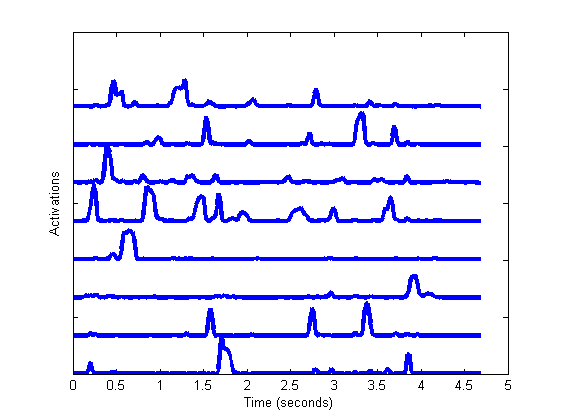
\includegraphics[width=.9\linewidth]{activations_machali}
  \captionof{figure}{Activation vectors for Machali}\label{activations_machali_nmf}
  \label{fig:test1}
\end{minipage}%
\begin{minipage}{.5\textwidth}
  \centering
  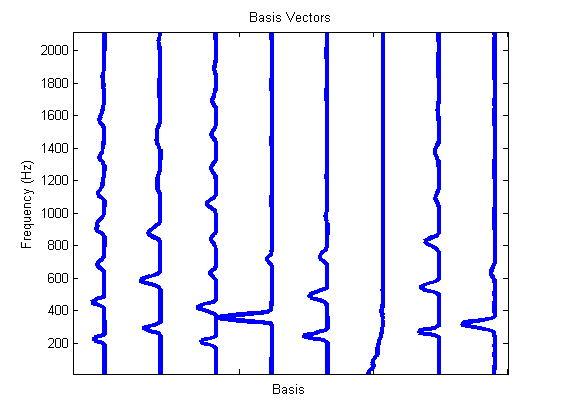
\includegraphics[width=.9\linewidth]{basis_vectors_machali}
  \captionof{figure}{Basis Vectors for machali}\label{basis_machami_nmf}
  \label{fig:test2}
\end{minipage}
\end{figure}


When reconstructing the speech audio  using NMF, although the error, $D$(KL divergence) is approximately equal, the audio reconstruction quality has several artifacts which is apparent on listening to the reconstructed audio\cite{A}. \\
Also, by looking at the basis vectors and activations, it is not possible to do an an intuitive analysis of the structure of the audio, as was done in the case of pure instrumental sounds in \emph{Mary}, partly because the activation patterns are much more complex and at many time instants, multiple basis vectors are activated.
The basis vectors also themselves do not reveal much about the speech spectrogram , and there is no apparent pattern in the activations that would indicate temporal patterns in the speech signal.
This calls for an extension to the conventional NMF by introducing a convolutive NMF model\cite{paris}\cite{grady}. Here, instead of each basis vector being a single spectrum, it is a series of consecutive spectra. The $W$ matrix, instead of being a 2-D matrix is a tensor of rank 3 of dimension $M \times R \times T$. The reconstruction in terms of W and H is now given as - 
\begin{align}
V \approx\sum_0^{T-1} W^T\stackrel{t\rightarrow}{H} \label{convnmf_eq}
\end{align}

The $t \rightarrow$ is the shift operator which represents shifting of the columns to the right by t steps. The updated multiplicative updates are as  given in \cite{paris}. T represents the length of each basis \emph{pattern}  (instead of basis \emph{vector}). By adding a temporal dimension to the basis vectors, they have been more expressive in terms of representing patterns in the spectrogram and help capture trends in the temporal dimension which were obscured in the activation vectors in the conventional NMF approach.

This convolutive version of the NMF was applied on the same audio, \emph{Machali}, and the results are shown in Figures 2.9-2.12 . They represent the spectrogram of the original audio, the reconstructed spectrogram, the activation matrix and the basis vectors respectively. All the parameters remained the same (Refer Figure 2.10) and the value of $T$ i.e. the length of each basis pattern was chosen to be 8 samples in the spectrogram domain, which, given the STFT parameters, translates to almost 0.17 seconds in the time domain. Although such a basis length is not entirely reasonable since speech is stationary only upto time segments of around 40ms, the choice is deliberately made for demonstration purposes.
\\
\begin{figure}
\centering
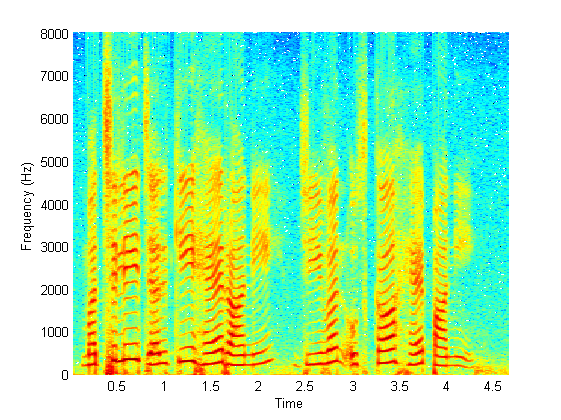
\includegraphics[scale=0.6]{machali_spectrogram}
\caption{Spectrogram of \emph{M}. Key STFT parameters - Sampling frequency : $16000kHz$. Window : hanning window of length 1024 samples. Overlap : 756 samples. Size of fft: 1024 }
\end{figure}

\begin{figure}
\centering
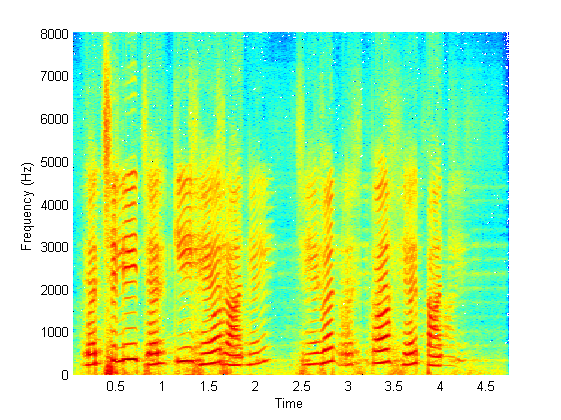
\includegraphics[scale=0.6]{machali_recon_spectrogram_c}
\caption{Reconstructed Spectrogram of \emph{Machali}. Key STFT parameters - R : 8, T = 8.Sampling frequency : $16000kHz$. Window : hanning window of length 1024 samples. Overlap : 756 samples. Size of fft: 1024 }
\end{figure}

\begin{figure}
\centering
\begin{minipage}{.5\textwidth}
  \centering
  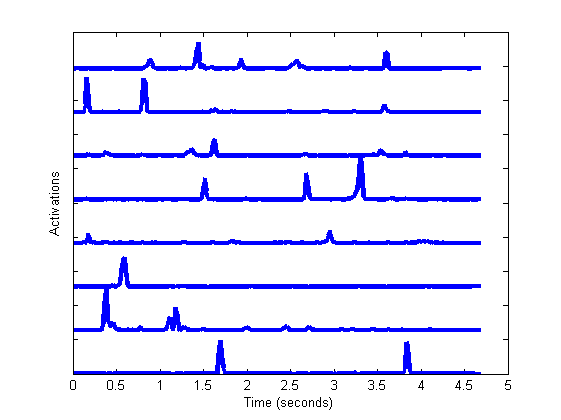
\includegraphics[width=.9\linewidth]{activations_machali_c}
  \captionof{figure}{Activations for Machali}
  \label{fig:test1}
\end{minipage}%
\begin{minipage}{.5\textwidth}
  \centering
  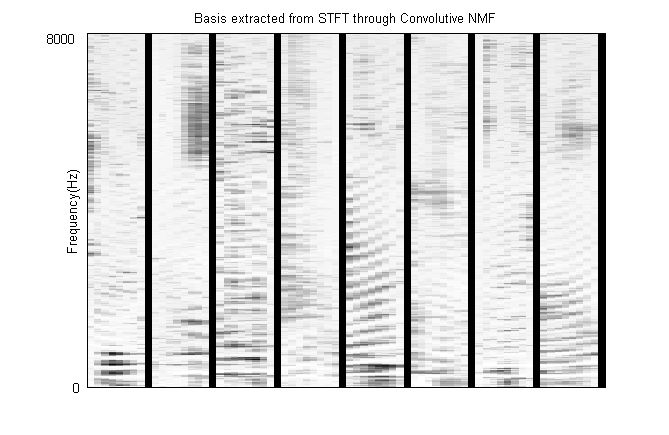
\includegraphics[width=.9\linewidth]{basis_machali_c}
  \captionof{figure}{Basis patterns for Machali}\label{convolutive_basis_machali}
  \label{fig:test2}
\end{minipage}
\end{figure}

The basis extracted using convolutive NMF are shown in Figure \ref{convolutive_basis_machali}. It is evident that the basis patterns say a lot more about the audio than their counterparts in in conventional NMF. Some of the bases look like spectrograms of speech phones in that they represent the harmonics with various pitch inflections. An audio reconstruction confirms that some basis patterns do represent specific speech phones\cite{A} Also, since the activation matrix is much more sparse in this case, when compared to that of the conventional NMF (Figure 2.7). This enables us to pinpoint the exact contribution of each basis to the spectrogram.
The convolutive model has more effectively captured the structure of speech and has provided a much more revealing set of basis objects. The performance of this technique relies heavily on the choice of the two key parameters - the number of basis($R$) and the time-length of each basis($T$). Not much work has been done regarding the choice of these parameters for a given signal. 
While it is intuitive that having more basis will always increase the accuracy of reconstruction, it also increases the time complexity of the decomposition and the marginal gain in accuracy may not be worth the complexity after a certain point.
Although the convolutivs NMF model does not do as well as NMF as far as reconstruction error is concerned, it has been employed in source separation \cite{paris} and dereverberation \cite{baby}. Thus, this representation for speech can be helpful in a few applications.
The next chapter will describe a popular approach for dereverberation through factorizing the magnitude spectrogram. 

